\section{System's Perspective}
\subsection{Architecture of your ITU-MiniTwit systems}
Below is a deployment diagram showing the system's architecture:
\begin{figure}[h!]
    \centering
    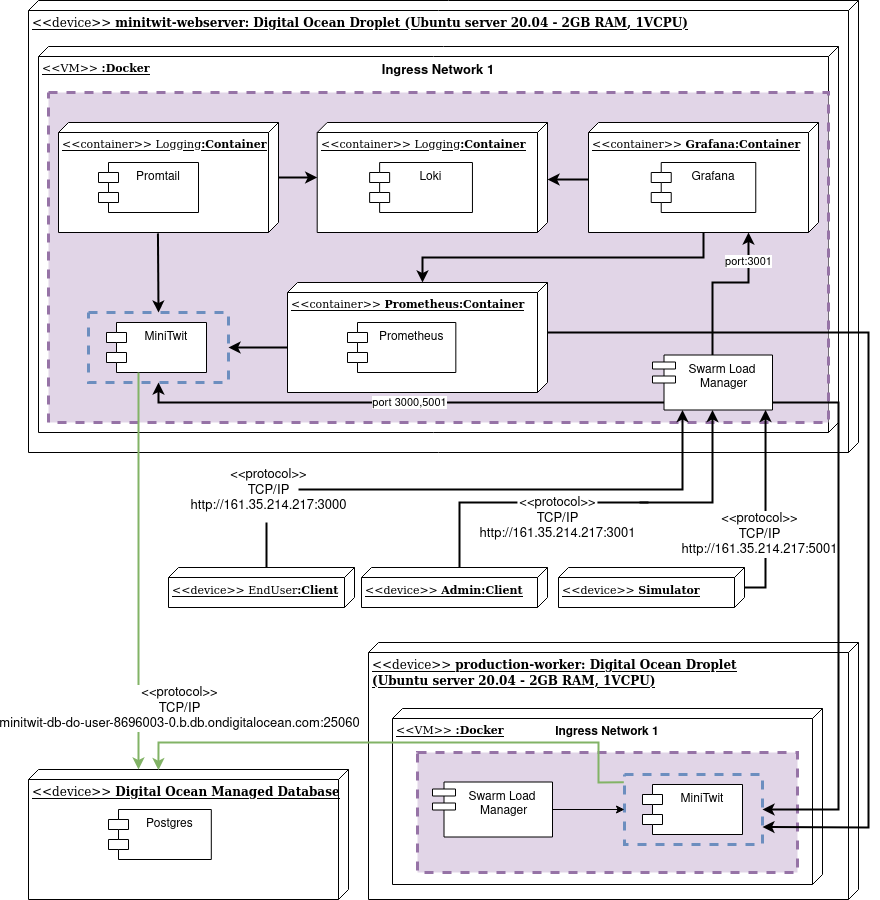
\includegraphics[width=1.2\linewidth]{report/images/system-architecture.png}
    \caption{System Architecture}
    \label{fig:arcitechture-overview}
\end{figure}

The MiniTwit application runs on two droplets on Digital Ocean. A managed database hosted by Digital Ocean is used to host a Postgres database. The \textit{manager-node-01} droplet is running Docker swarm mode and is the swarm manager and leader\cite{docker-swarm}. The \textit{workder-node-01} is a worker node within the swarm. The MiniTwit application itself is grouped into the Minitwit component. The swarm hosts the Minitwit component in two replica. The swarm also hosts monitoring and logging services each in one replica. The monitoring and logging stack consists of Promtail to perform log aggregation, Loki to store and enable log query, Prometheus to collect and perform metric querying and finally Grafana to display the monitored and logged data. \\
\\
Below is a decomposition of the Minitwit component:

\begin{figure}[h!]
    \centering
    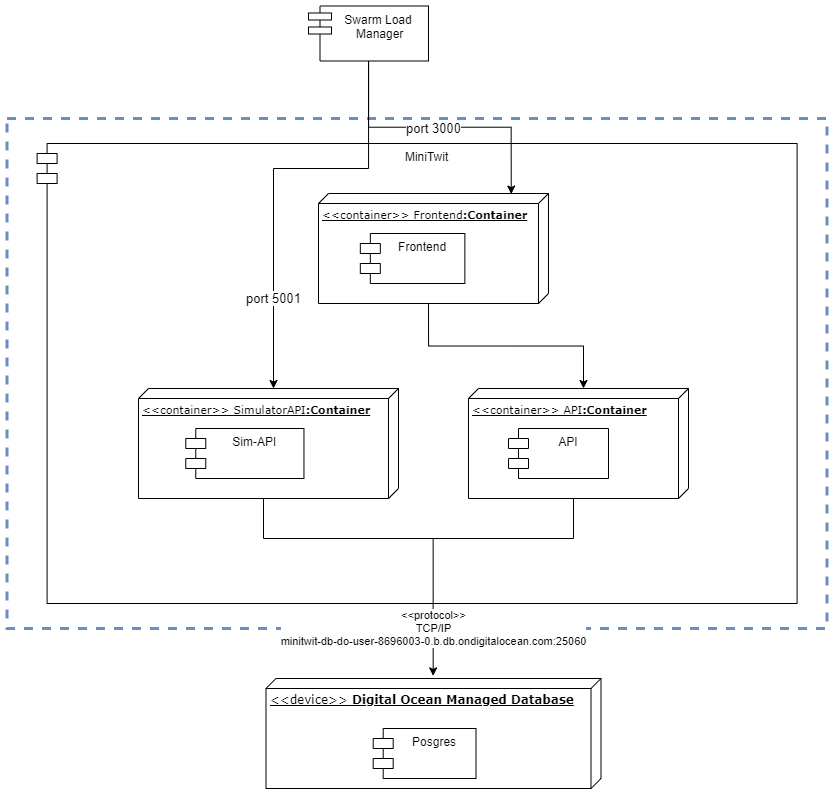
\includegraphics[width=1\linewidth]{report/images/minitwit-decomposition.png}
    \caption{MiniTwit Component Decomposition}
    \label{fig:arcitechture-overview}
\end{figure}

The Minitwit component is an abstraction to increase readability in the UML drawing and is therefore not a single container hosted in the swarm. The component consists of the front-end, API for the simulator (Sim-Api) and the API for the front-end.

\subsection{Design of your ITU-MiniTwit systems}
The \textit{Frontend} is written in React JS. Both the \textit{Sim-API} and \textit{API} are written in Node.js using ExpressJS and implemented as a RESTful API. 
\todo{hvad skal der egentligt stå her???}

\subsection{All dependencies of your ITU-MiniTwit systems on all levels of abstraction and development stages.}
\subsubsection{That is, list and briefly describe all technologies
and tools you applied and depend on.}
\todo{Hvad søren mener i TAs?}
\subsection{Important interactions of subsystems}
\todo{Nu er det her ikke danmarkskortet, så hvad mener i? Er det hvordan de enkelte klasser snakker sammen eller på et komponent niveau?}
\subsection{Describe the current state of your systems, for example using results of static analysis and quality assessment systems.}
\subsection{Finally, describe briefly, if the license that you have chosen for your project is actually compatible with the licenses of all your direct dependencies.}